\documentclass[dvipdfmx,twocolumn]{jsarticle}
\usepackage{cs-handout}

% フォント関連
\usepackage[T1]{fontenc}
\usepackage{otf}

% 便利なパッケージ
\usepackage{graphicx}
\usepackage{xcolor}
\usepackage{booktabs}
\usepackage{url}
\usepackage{enumitem}
\usepackage{hyperref}
\usepackage{pxjahyper}
\usepackage{amsmath,amssymb}
\usepackage{lipsum} % ダミーテキスト生成用
\usepackage{fancyhdr}
\usepackage[skip=0pt]{caption}  % ← これをプリアンブルに追加
\captionsetup{font=small}
\usepackage{enumitem}
\setlist{nolistsep}
\usepackage{multirow}
\usepackage{array}
\usepackage{float}
\usepackage{here}

\usepackage{pgffor}
\newcommand{\RepeatPlaceholder}[2]{\textcolor{gray}{\foreach\x in {1,...,#1}{#2}}}
\newcommand{\Note}[1]{\noindent \textbf{\textcolor{blue}{#1}}}

% 著者情報
\title{エンタープライズ無線LAN環境における\\通信品質改善のためのユーザ行動支援手法}
\author{上川雅弘}
\studentid{2210182}
\office{矢崎研究室} % 〇〇〇〇は主任指導教員名

% 発表会情報
%\lhead{\arabic{academicyear}年度 情報理工学研究科 情報・ネットワーク工学専攻 CSプログラム 修士論文発表会}
%\lhead{\arabic{academicyear}年度 情報理工学研究科 情報・ネットワーク工学専攻 CSプログラム 修士論文中間発表会}
%\lhead{\arabic{academicyear}年度9月期 情報理工学研究科 情報・ネットワーク工学専攻 CSプログラム 修士論文発表会}
%\lhead{\arabic{academicyear}年度9月期 情報理工学研究科 情報・ネットワーク工学専攻 CSプログラム 修士論文中間発表会}
\lhead{\arabic{academicyear}年度 情報理工学域 I類 CSプログラム 卒業研究発表会}
%\lhead{\arabic{academicyear}年度 情報理工学域 I類 CSプログラム 卒業研究中間発表会}
\presentationdate{2025}{7}{30} % 発表会の日付

\begin{document}
\maketitle

\section{はじめに}
%\Note{研究ストーリー(このフォントはコメント)}
企業や大学における統合管理された無線LAN環境(エンタープライズ無線LAN環境)では,多くのユーザが同時に接続することが一般的となっているが,そこではしばしば通信品質が低下する.
こうした問題は業務効率や学習環境を直接的に低下させるだけでなく,利用者が体感するQoE(Quality of Experience)にも悪影響を及ぼす.
そのため,無線LAN環境の安定性は情報通信インフラとしての信頼性を左右する重要な課題である.
従来,これらの課題に対しては,ネットワーク管理者がアクセスポイント(AP)の配置を最適化したり,チャネルの割り当てを調整したりすることで対応してきた.
しかし,管理者の努力だけでは完全に制御できない要因も数多く存在する.
そこで本研究では,従来の管理者主体のアプローチとは異なり,利用者自身の行動に着目した新しい通信品質改善手法を提案した~\cite{kamikawa2025}.本稿では,シミュレーションによる結果とその評価を報告する.
\section{関連研究}
%\Note{参考文献はすべて本文中で適切に引用すべし:
利用者側に着目したアプローチとして,Miyataらの研究~\cite{Miyata2012}がある.
この研究では,ユーザが積極的に移動して通信品質を改善する手法が提案されているが,実際の利用シーンでは大きな移動は困難である場合が多い.
一方,本研究では,ユーザの負担を最小限に抑えるために,消極的な移動を前提とした手法を提案している.
\section{背景}
%\Note{前提知識の説明}
\subsection{QoEとスループット}
利用者のQoEにとってスループットは重要な指標である.
これが低下すると,インターネット利用に支障が生じ,利用者の満足度も低下する.
スループットは単純にAPと端末との距離に依存するだけでなく,接続端末数や無線チャネルの混雑度にも影響を受ける.
同じ距離条件であっても,APに多数のユーザが集中している場合や,利用しているチャネルが他の電波で占有されている場合には,スループットは低下する.
\subsection{チャネル使用率}
チャネル使用率とは,あるチャネルが単位時間あたりにどの程度の割合占有されているかを示す指標である.
値が高いほど,そのチャネルでは多数の通信が同時に行われていることを意味し,スループットが低下する傾向にある.
本研究では,QoEをスループットで評価しつつ,チャネル使用率を考慮することで,より実環境に即した分析と手法設計を行う.
\section{提案}
%\Note{提案内容の説明}
本研究では,従来のアプローチの限界を踏まえ,ユーザの負担を最小限に抑えながら通信品質を改善するための新しい支援手法を提案する.
特徴は,消極的な移動を前提とし,利用者に大きな移動を強いずにQoEの改善を目指す.
\subsection{基本方針}
ユーザは自身の移動可能距離$d_{th}$と,通信に必要な最低限のスループット要求値$\theta_{th}$を入力として与える.
システムはこれをもとに,候補となるAPの集合を抽出する.
その後,各候補APに対して通信環境を総合的に評価し,最適な接続先および移動先を提案する.
\subsection{処理フロー}
まず,ユーザからの入力$d_{th}$と$\theta_{th}$を受け取る.
次に,ユーザの移動前の位置から距離$d_{th}$以内に存在するAPの集合を候補APとして抽出する.
さらに,各候補APに対し,システムを使用するユーザが接続した場合のスループットを試算する.
その後,ユーザが各候補APに対し以下の指標を正規化しスコア化する.
\begin{itemize}[noitemsep, topsep=0pt]
  \item スループット
  \item チャネル使用率
  \item ユーザとの距離
  \item 接続中のユーザ数
\end{itemize}
これらの各スコアに重みをつけて加重平均をとる.
総合スコア上位APの中から,全体スループットを最大化するAP$a$と移動ベクトル$m$を選定し,ユーザに提示する.

% \begin{figure}[tb]
%  \centering
%  \includegraphics[width=\linewidth]{example-image-a}
%  \caption{\Note{図のキャプションは下}}
% \end{figure}

\section{評価}
%\Note{提案に対する評価}
提案手法の有効性を検証するために,ネットワークシミュレータ ns-3.35 を用いてシミュレーション実験を行った.
実験では,異なる環境条件やユーザ数を設定し,従来のランダム移動との比較を通じて,提案手法がシステム全体のスループット改善にどの程度寄与するかを評価した.
\subsection{シミュレーション設定}
シミュレーションは,図1のように,50m四方の仮想空間にAPを複数配置し,既存ユーザと新規ユーザが混在する状況を想定して実施した.
\begin{figure}[H]
  \centering
  \vspace{-4mm} % 図の上の余白を削る
  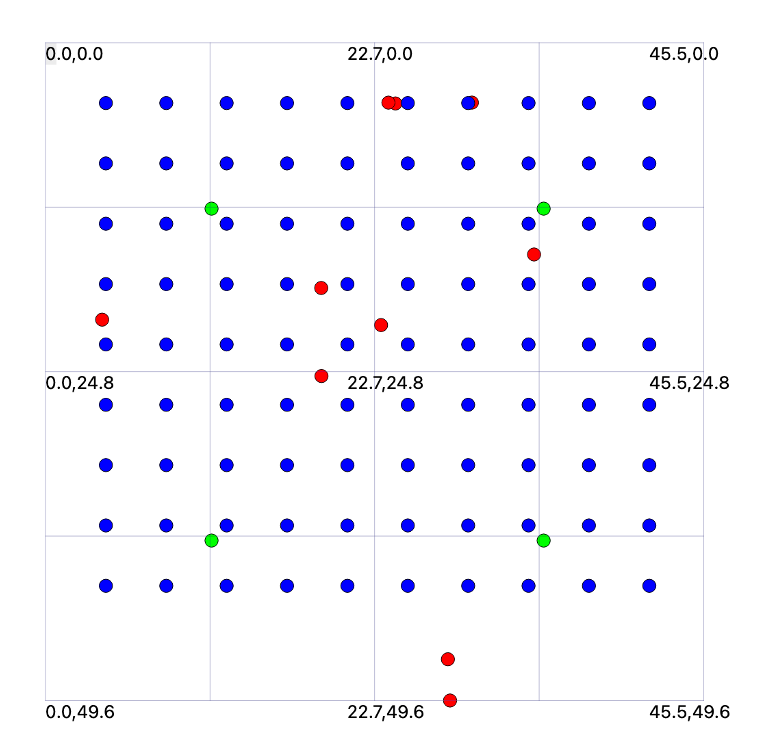
\includegraphics[width=0.8\linewidth]{simulation.png}
  \vspace{-2mm} % 図とキャプションの間を詰める
  \caption{シミュレーション結果}
  \vspace{-9mm} % キャプション下の余白を削る
\end{figure}
今回のケースでは4台のAPをランダムに配置した.このAPのWi-Fi規格は802.11ax-2.4GHzとし,チャネルはそれぞれ別のものを1つずつを割り当てた.
それぞれのAPには異なるチャネル使用率を設定し,環境における混雑度の違いを再現した(例:AP0=0.2, AP1=0.3, AP2=0.4, AP3=0.5)。
初期状態では90人の既存ユーザを等間隔に配置し,さらに新たに10人のユーザが環境内に参加するケースを想定した.
新規ユーザは$d_{th}=15[m]$の範囲内で移動できるとし,要求スループットは30Mbpsに設定した.
各シナリオは100回繰り返し実施し,結果のばらつきを抑えるために平均値を算出した.
各試行のシミュレーション時間は30秒とした.
評価の指標としては,システム全体のスループットについて,新規ユーザが移動しなかった場合に比べてどの程度改善したかを示す値(改善率)及び移動距離の分布を採用した.
\subsection{シミュレーション結果}
図2に示すように,提案手法は従来手法に比べ,スループットが2.69\%向上した.
\begin{figure}[H]
 \centering
 \vspace{-5mm} % 図の上の余白を削る
 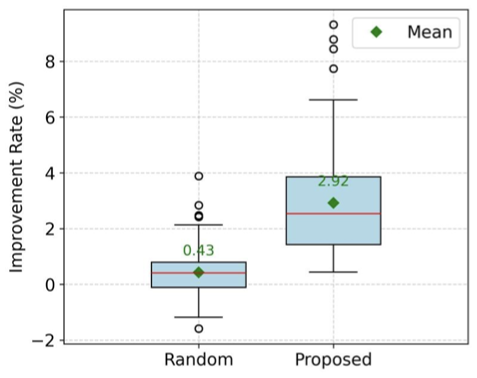
\includegraphics[width=0.8\linewidth]{boxplot_50_50.png}
  \vspace{-2mm} % 図とキャプションの間を詰める
 \caption{{改善率}}
  \vspace{-6mm} % キャプション下の余白を削る
\end{figure}
\begin{figure}[H]
 \centering
  \vspace{-5mm} % 図の上の余白を削る
 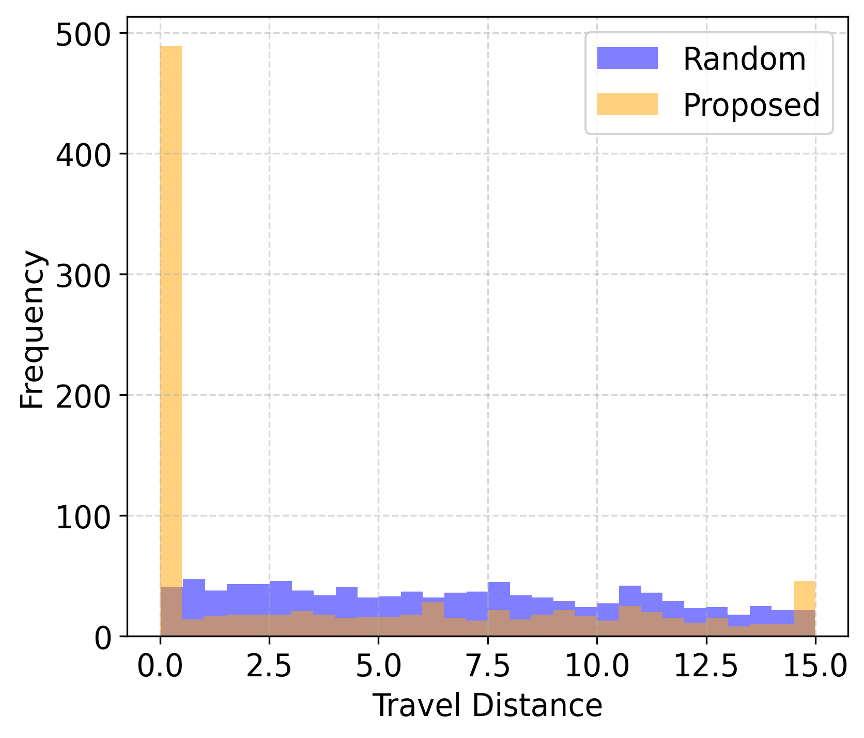
\includegraphics[width=0.8\linewidth]{hist.png}
  \vspace{-2mm} % 図とキャプションの間を詰める
 \caption{{移動距離の分布}}
  \vspace{-6mm} % キャプション下の余白を削る
\end{figure}
また,移動距離の観点では,多くのユーザが5m未満の小規模な移動で十分な改善を得られており,過度な行動負担を課すことなくQoE向上が可能であることが示された.
一方で,初期位置が極端に不利なユーザについては,15m移動しても要求スループットを満たせないケースも一定数存在した.この点は今後の課題として追加的な対策が必要である.
% \begin{table}[tb]
%  \centering
%  \caption{\Note{表のキャプションは上}}
%  \vspace{-\bigskipamount}
%  \begin{tabular}[t]{ll}
%   \toprule
%   パッケージ名 & 説明 \\ \midrule
%   graphicx & 画像を挿入する \\
%   xcolor & 色を指定する \\
%   booktabs & このスタイルの表を記述する \\
%   url & URL \url{uec.ac.jp} を記述する \\
%   hyperref & URL をハイパーリンクにする \\
%   pxjahyper & hyperrefの日本語向け調整 \\
%   \bottomrule
%  \end{tabular}
% \end{table}

\section{おわりに}
%\Note{まとめと今後の課題}
本研究では,エンタープライズ無線LAN環境における通信品質のばらつきに対し,利用者の消極的移動を活用した新しい支援手法を提案した.
提案手法は,スループット・チャネル使用率・移動距離・既存ユーザ数の4指標を組み合わせてAPを評価し,最適な接続先を決定する.
シミュレーションにより,ランダム移動と比較してシステム全体のスループットが平均2.92%改善し,移動距離も抑制できることを確認した.
今後の課題としては,実環境での検証や,先行研究との比較,ユーザが正確かつ簡単に自身の位置を申告する仕組みの考案が挙げられる.

\bibliographystyle{jplain}
\bibliography{ref}
%\Note{pBibTeXの利用を推奨}

\end{document}
